\documentclass[conference]{IEEEtran}

\usepackage{amsmath,amssymb,amsfonts,bm}
\usepackage{graphicx}
\usepackage{booktabs}
\usepackage{array}
\usepackage{multirow}
\usepackage{xcolor}
\usepackage{cite}
\usepackage{url}

\title{Nonlinear Trajectory Optimization for Swing-Up of a Double Inverted Pendulum on a Cart}

\author{
\IEEEauthorblockN{Author Name}
\IEEEauthorblockA{Department of Mechanical and Aerospace Engineering\\
Course Project Report}
}

\begin{document}
\maketitle

\begin{abstract}
This paper presents a detailed implementation-oriented description of the CasADi-based nonlinear trajectory optimization module used for a double inverted pendulum on a cart. Unlike the MPPI controller, which replans online in closed loop, the method studied here formulates the task as a finite-horizon open-loop optimal control problem and solves it by direct multiple shooting. The state trajectory, control sequence, dynamic constraints, path cost, terminal cost, initialization strategy, and solver configuration are documented exactly as implemented in the code. The system is modeled as a six-state, single-input underactuated nonlinear mechanism with two point-mass links attached to a translating cart. A smooth swing reference and a feedforward input guess are used to initialize the nonlinear program, while symbolic RK4 integration enforces dynamic consistency over the horizon. The resulting formulation provides a compact and readable example of how modern nonlinear optimization tools can be applied to swing-up planning for an underactuated robotic benchmark. In the verified default run with CasADi and IPOPT available, the optimizer produced a feasible swing-up plan whose terminal cart-position error was approximately $0.047$~m and whose terminal angle errors were approximately $1.7\times10^{-3}$~rad and $-2.3\times10^{-3}$~rad, although nonzero terminal velocities remained.
\end{abstract}

\begin{IEEEkeywords}
trajectory optimization, direct multiple shooting, CasADi, nonlinear optimal control, double inverted pendulum, cart-pole
\end{IEEEkeywords}

\section{Introduction}
The double inverted pendulum on a cart is a representative underactuated system in which one horizontal actuator must generate coordinated motion across multiple unstable degrees of freedom. In such systems, the control objective is not simply to reject small perturbations around an equilibrium. Instead, the controller or planner must deliberately create large transient motion, exploit nonlinear coupling, and steer the system into a stabilizable neighborhood of the upright configuration. This is precisely the type of problem for which nonlinear trajectory optimization is attractive.

Trajectory optimization differs from online sampling control in both purpose and structure. Rather than repeatedly recomputing a short-horizon corrective policy during execution, the optimizer seeks a full finite-horizon state and control plan that satisfies the nonlinear dynamics and minimizes a designed objective. Once such a plan is found, it can be visualized directly as an optimized state trajectory or replayed as an open-loop control sequence on the original nonlinear simulator. The present repository includes both of these options.

The goal of this paper is to document that trajectory optimization implementation as a standalone technical report. The emphasis is on what is actually encoded in the software: the state convention, the manipulator-form model, the reference generation method, the direct multiple-shooting transcription, the exact weights in the objective, the optional track-bound constraints, the solver-selection logic, and the interpretation of the resulting plan. The paper is written so that a reader could reconstruct the optimization problem from the manuscript alone.

To make the manuscript readable even for someone who has not recently worked with trajectory optimization, terminology is introduced gradually and repeated when needed. In particular, whenever a compact equation is presented, the variables in that equation are explained in words immediately afterward rather than being left implicit.

\section{Modeling and Problem Setup}
\subsection{Coordinates, State, and Control}
Let the generalized coordinates be
\begin{equation}
\bm{q} = \begin{bmatrix} x & \theta_1 & \theta_2 \end{bmatrix}^\top,
\end{equation}
where $x$ is the cart position and $\theta_1,\theta_2$ are the first and second link angles measured from the upright direction. Thus the upright equilibrium is at
\begin{equation}
\theta_1 = \theta_2 = 0,
\end{equation}
while a hanging configuration is near
\begin{equation}
\theta_1 = \theta_2 = \pi.
\end{equation}
The complete state vector is
\begin{equation}
\bm{x} = \begin{bmatrix} x & \theta_1 & \theta_2 & \dot{x} & \dot{\theta}_1 & \dot{\theta}_2 \end{bmatrix}^\top \in \mathbb{R}^6,
\end{equation}
and the scalar control input is the horizontal cart force
\begin{equation}
u \in \mathbb{R}.
\end{equation}
Here the term \emph{generalized coordinates} simply means the minimal coordinates used to describe the configuration of the mechanism. In this problem, $x$ describes the horizontal position of the cart, while $\theta_1$ and $\theta_2$ describe the orientations of the two pendulum links. The symbol $\bm{q}$ therefore captures configuration only, whereas the full state $\bm{x}$ includes both configuration and velocity.

The default parameter set in the repository is
\begin{align}
m_0 &= 1.0 \text{ kg}, &
m_1 &= 0.2 \text{ kg}, &
m_2 &= 0.2 \text{ kg}, \\
l_1 &= 0.5 \text{ m}, &
l_2 &= 0.5 \text{ m}, &
g &= 9.81 \text{ m/s}^2,
\end{align}
with cart damping $d_x=0.1$, joint damping $d_1=d_2=0.02$, and force limit $u_{\max}=30$~N in the default model.

The damping terms $d_x$, $d_1$, and $d_2$ are viscous damping coefficients. ``Viscous'' here means that the corresponding resistive force or torque is proportional to velocity. The parameter $u_{\max}$ is the actuator saturation limit: even if the optimizer asks for a larger force, the dynamics clip it to this bound.

\subsection{Kinematic Convention}
Each pendulum link is modeled as a rigid, massless rod with a point mass at its tip. The cart position is
\begin{equation}
\bm{p}_c = \begin{bmatrix} x \\ 0 \end{bmatrix},
\end{equation}
the first tip position is
\begin{equation}
\bm{p}_1 = \bm{p}_c + \begin{bmatrix} l_1 \sin\theta_1 \\ l_1 \cos\theta_1 \end{bmatrix},
\end{equation}
and the second tip position is
\begin{equation}
\bm{p}_2 = \bm{p}_1 + \begin{bmatrix} l_2 \sin\theta_2 \\ l_2 \cos\theta_2 \end{bmatrix}.
\end{equation}
This global-angle representation is simple to visualize and is consistent with the rest of the code base. It also means that angle differences in the cost should be handled through periodic functions rather than naive Euclidean subtraction alone.

The notation $\bm{p}_c$, $\bm{p}_1$, and $\bm{p}_2$ denotes Cartesian positions in the plane. The subscript $c$ stands for cart, while the subscripts $1$ and $2$ denote the tip of the first and second links. These positions are not only useful for drawing the mechanism; they also help explain why the problem is underactuated. The only direct actuator acts on the cart, and the pendulum links move only through the geometric and inertial coupling induced by the cart motion.

\subsection{Dynamic Model}
The implemented dynamics take the form
\begin{equation}
\bm{M}(\bm{q}) \ddot{\bm{q}} = \bm{\tau}(\bm{q},\dot{\bm{q}},u),
\label{eq:manip}
\end{equation}
In this equation, $\bm{M}(\bm{q})$ is the configuration-dependent mass matrix, $\ddot{\bm{q}}$ is the generalized acceleration vector, and $\bm{\tau}(\bm{q},\dot{\bm{q}},u)$ collects all generalized forces and torques, including control input, damping, gravity, and velocity-coupling terms. Writing the model in this form is common in robotics because it separates inertia from the remaining forces.
with mass matrix
\begin{equation}
\bm{M}(\bm{q}) =
\begin{bmatrix}
m_0 + m_1 + m_2 & (m_1+m_2)l_1\cos\theta_1 & m_2l_2\cos\theta_2 \\
(m_1+m_2)l_1\cos\theta_1 & (m_1+m_2)l_1^2 & m_2l_1l_2\cos(\theta_1-\theta_2) \\
m_2l_2\cos\theta_2 & m_2l_1l_2\cos(\theta_1-\theta_2) & m_2l_2^2
\end{bmatrix},
\end{equation}
and generalized forces
\begin{align}
\bm{\tau} =
\begin{bmatrix}
u - d_x \dot{x} + (m_1+m_2)l_1\sin\theta_1 \dot{\theta}_1^2 + m_2l_2\sin\theta_2 \dot{\theta}_2^2 \\
-d_1 \dot{\theta}_1 - m_2l_1l_2\sin(\theta_1-\theta_2)\dot{\theta}_2^2 + (m_1+m_2)gl_1\sin\theta_1 \\
-d_2 \dot{\theta}_2 + m_2l_1l_2\sin(\theta_1-\theta_2)\dot{\theta}_1^2 + m_2gl_2\sin\theta_2
\end{bmatrix}.
\end{align}
The first row and column of $\bm{M}(\bm{q})$ correspond to the cart coordinate, while the second and third rows and columns correspond to the two angular coordinates. The off-diagonal terms are important: they encode coupling between cart motion and link motion, and also between the two links themselves. In the force vector $\bm{\tau}$, the term $u-d_x\dot{x}$ is the net horizontal actuation on the cart, the terms containing $\sin(\theta_i)\dot{\theta}_i^2$ are centrifugal-type effects, the terms proportional to $g$ are gravity contributions, and the terms proportional to $d_1$ and $d_2$ are viscous joint damping torques.

Solving \eqref{eq:manip} yields $\ddot{\bm{q}}$, and the first-order state dynamics become
\begin{equation}
\dot{\bm{x}} = \bm{f}(\bm{x},u)
=
\begin{bmatrix}
\dot{x} & \dot{\theta}_1 & \dot{\theta}_2 & \ddot{x} & \ddot{\theta}_1 & \ddot{\theta}_2
\end{bmatrix}^\top.
\end{equation}
The notation $\bm{f}(\bm{x},u)$ is standard in control: it denotes the time derivative of the state as a function of the current state and input. Once this first-order form is available, it can be used by numerical integrators, trajectory optimizers, or feedback controllers without changing the physical model itself.

The control is clipped to the admissible range before entering the dynamics:
\begin{equation}
u_{\mathrm{sat}} = \mathrm{clip}(u,-u_{\max},u_{\max}).
\end{equation}
The symbol $u_{\mathrm{sat}}$ means \emph{saturated control input}. The function $\mathrm{clip}(\cdot)$ truncates the input so that it remains inside the admissible interval $[-u_{\max},u_{\max}]$. This models a real actuator that cannot produce arbitrarily large force.

\subsection{Task Definition}
The default trajectory-optimization demo sets
\begin{equation}
\bm{x}_0 = \begin{bmatrix} 0 & \pi + 0.08 & \pi - 0.08 & 0 & 0 & 0 \end{bmatrix}^\top
\end{equation}
as the initial state and
\begin{equation}
\bm{x}^\star = \begin{bmatrix} 3 & 0 & 0 & 0 & 0 & 0 \end{bmatrix}^\top
\end{equation}
as the target state. The default discretization uses $N=40$ multiple-shooting intervals with $\Delta t = 0.08$~s, corresponding to a planning horizon of $3.2$~s.

An optional cart-position bound
\begin{equation}
x \in [x_{\min},x_{\max}] = [-2.5,5.5]
\end{equation}
can also be enforced inside the nonlinear program. However, the script explicitly disables this by default because the fallback \texttt{sqpmethod} backend often struggles when the hard bounds are active.
The notation $x \in [x_{\min},x_{\max}]$ simply means that the cart position is restricted to lie between a lower bound $x_{\min}$ and an upper bound $x_{\max}$. Such a bound is often called a \emph{box constraint} because it restricts a variable to an interval.

\section{Reference Generation and Initialization}
\subsection{Smooth Swing Reference}
The optimizer is warm-started using a smooth state reference built by interpolating the initial and goal states. Let
\begin{equation}
\tau_k = \frac{k}{N}, \qquad k=0,\ldots,N,
\end{equation}
and define the cubic smoothstep profile
\begin{equation}
s(\tau) = 3\tau^2 - 2\tau^3.
\end{equation}
Here $k$ is the discrete stage index along the planning horizon, and $N$ is the total number of shooting intervals. The variable $\tau_k$ is therefore a normalized time index that moves from $0$ at the start of the horizon to $1$ at the end. The function $s(\tau)$ is a smooth interpolation profile. It starts at $0$, ends at $1$, and has zero slope at both endpoints, which makes it gentler than a straight-line interpolation.

Then the initialization reference is
\begin{align}
x_k^{\mathrm{ref}} &= x_0 + (x^\star - x_0)s(\tau_k), \\
\theta_{1,k}^{\mathrm{ref}} &= \theta_{1,0} + (\theta_1^\star - \theta_{1,0})s(\tau_k), \\
\theta_{2,k}^{\mathrm{ref}} &= \theta_{2,0} + (\theta_2^\star - \theta_{2,0})s(\tau_k),
\end{align}
while the velocity components of the reference are set to zero:
\begin{equation}
\dot{x}_k^{\mathrm{ref}} = \dot{\theta}_{1,k}^{\mathrm{ref}} = \dot{\theta}_{2,k}^{\mathrm{ref}} = 0.
\end{equation}
The superscript ``ref'' stands for \emph{reference}. Thus $x_k^{\mathrm{ref}}$ is the reference cart position at stage $k$, and $\theta_{1,k}^{\mathrm{ref}}$, $\theta_{2,k}^{\mathrm{ref}}$ are the reference link angles at the same stage. These quantities are not optimized directly; instead, they are used to initialize and shape the optimization.

This reference is not meant to satisfy the dynamics. Instead, it serves as a meaningful initial guess and as a shaping target inside the path cost. Using a smooth interpolation rather than a linear one avoids sharp endpoint slopes and provides a more natural state initialization for the nonlinear program.
The term \emph{warm start} refers to this practice of initializing the solver with a nontrivial guess rather than zeros or random values. Warm starting can significantly improve convergence, especially in nonlinear problems where a poor initial guess may lead the solver toward an undesirable local solution or slow progress.

\subsection{Feedforward Input Guess}
For each reference state, the code computes a scalar feedforward control guess by minimizing the squared acceleration magnitude:
\begin{equation}
u_k^{\mathrm{ref}} \in \arg\min_{u \in [-u_{\max},u_{\max}]} \left\| \ddot{\bm{q}}(\bm{x}_k^{\mathrm{ref}},u) \right\|_2^2.
\label{eq:ff}
\end{equation}
The expression $\arg\min$ means ``the value of the decision variable that minimizes the expression on the right.'' In this case, the decision variable is the scalar force $u$, and the objective is the squared Euclidean norm of the generalized acceleration vector $\ddot{\bm{q}}$. The notation $\|\cdot\|_2$ denotes the standard Euclidean norm. Therefore, \eqref{eq:ff} chooses a force that makes the reference state as dynamically quiet as possible, in the sense of minimizing total squared acceleration.

In the implementation, this is done with a bounded scalar optimization routine. Intuitively, \eqref{eq:ff} chooses a control that makes the reference state ``as close as possible'' to a force-balanced configuration, even though the full reference trajectory is not exactly dynamically feasible.

This feedforward initialization plays two roles. First, it improves numerical convergence by giving the solver a control trajectory that is less arbitrary than all zeros. Second, it allows the cost to regularize the optimized control around something physically interpretable rather than around the origin alone.

\IfFileExists{../figures/trajopt_reference.pdf}{
\begin{figure}[t]
\centering
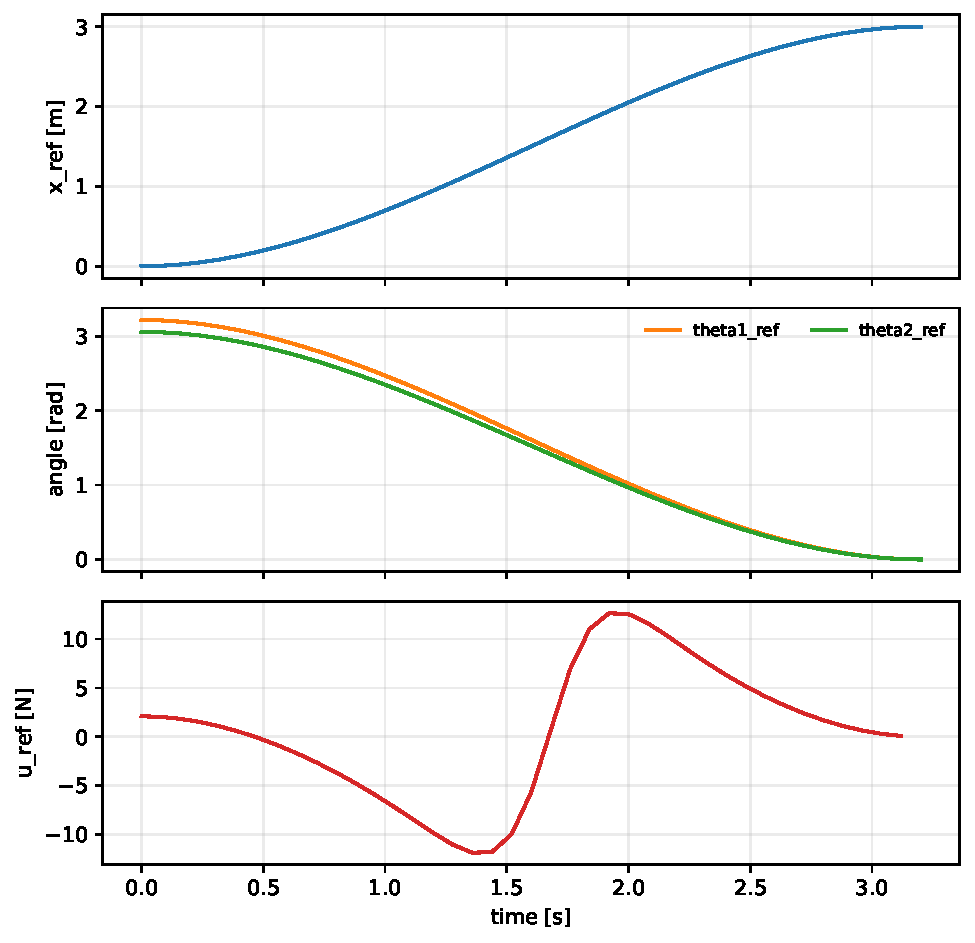
\includegraphics[width=\columnwidth]{../figures/trajopt_reference.pdf}
\caption{Smooth reference and feedforward input initialization used to warm-start the trajectory optimization problem for the default $N=40$, $\Delta t=0.08$ setup.}
\label{fig:refinit}
\end{figure}
}{
\begin{figure}[t]
\centering
\fbox{\parbox{0.95\columnwidth}{\centering
Reference-initialization figure placeholder.}}
\caption{Placeholder for the reference and feedforward initialization plot.}
\label{fig:refinit}
\end{figure}
}

\section{Direct Multiple-Shooting Formulation}
\subsection{Decision Variables}
The nonlinear program is built in CasADi through an \texttt{Opti} object. The optimization variables are
\begin{equation}
\bm{X} = \begin{bmatrix}\bm{x}_0 & \bm{x}_1 & \cdots & \bm{x}_N\end{bmatrix} \in \mathbb{R}^{6 \times (N+1)}
\end{equation}
and
\begin{equation}
\bm{U} = \begin{bmatrix}u_0 & u_1 & \cdots & u_{N-1}\end{bmatrix} \in \mathbb{R}^{1 \times N}.
\end{equation}
The matrix $\bm{X}$ stacks all state variables across the horizon. Each column is one \emph{shooting node state}, meaning the state at one discrete point along the horizon. Likewise, $\bm{U}$ stacks all control variables. In trajectory optimization, the variables are not just the current state and current input; the entire state and control sequence over the planning horizon is optimized together.

Although $\bm{x}_0$ is part of the variable matrix, it is constrained to equal the prescribed initial state:
\begin{equation}
\bm{x}_0 = \bm{x}_{\mathrm{init}}.
\end{equation}
The symbol $\bm{x}_{\mathrm{init}}$ denotes the known initial condition supplied by the user or script. Including $\bm{x}_0$ inside the optimization matrix but constraining it to this value is a common implementation pattern because it keeps the state array structurally uniform from stage $0$ through stage $N$.

\subsection{Symbolic RK4 Defect Constraints}
Dynamic feasibility is enforced through direct multiple shooting. For each stage $k=0,\ldots,N-1$, the next state variable is constrained to equal one RK4 step of the symbolic dynamics:
\begin{equation}
\bm{x}_{k+1} = \Phi_{\mathrm{RK4}}(\bm{x}_k,u_k),
\label{eq:defect}
\end{equation}
The phrase \emph{direct multiple shooting} means that the state at every stage is treated as an optimization variable, and dynamic consistency is imposed by constraints between neighboring stages. The map $\Phi_{\mathrm{RK4}}(\bm{x}_k,u_k)$ means ``the state obtained after one Runge--Kutta 4 integration step starting from $\bm{x}_k$ under input $u_k$.'' The constraints in \eqref{eq:defect} are often called \emph{defect constraints} because they force the difference between the left and right sides to be zero.

where $\Phi_{\mathrm{RK4}}$ is defined by
\begin{align}
\bm{k}_1 &= \bm{f}(\bm{x}_k,u_k), \\
\bm{k}_2 &= \bm{f}\!\left(\bm{x}_k+\frac{\Delta t}{2}\bm{k}_1,u_k\right), \\
\bm{k}_3 &= \bm{f}\!\left(\bm{x}_k+\frac{\Delta t}{2}\bm{k}_2,u_k\right), \\
\bm{k}_4 &= \bm{f}\!\left(\bm{x}_k+\Delta t \bm{k}_3,u_k\right), \\
\Phi_{\mathrm{RK4}}(\bm{x}_k,u_k) &= \bm{x}_k + \frac{\Delta t}{6}\left(\bm{k}_1 + 2\bm{k}_2 + 2\bm{k}_3 + \bm{k}_4\right).
\end{align}
In this RK4 formula, $\bm{k}_1,\bm{k}_2,\bm{k}_3,\bm{k}_4$ are intermediate slope evaluations of the state derivative. The parameter $\Delta t$ is the timestep between two neighboring shooting nodes. RK4 is a fourth-order integration method, meaning that it is considerably more accurate than forward Euler for the same timestep, while still being simple enough to embed symbolically inside an optimizer.

The defect constraints in \eqref{eq:defect} are central to the method. They allow every shooting node state to be a decision variable while ensuring that adjacent nodes remain dynamically consistent. Relative to single shooting, this generally improves numerical conditioning because the optimizer can adjust intermediate states directly rather than only through the control sequence.

\subsection{Box Constraints}
The optimizer imposes the control bounds
\begin{equation}
-u_{\max} \le u_k \le u_{\max}, \qquad k=0,\ldots,N-1.
\end{equation}
This inequality means that every stage input $u_k$ must remain inside the actuator range. The subscript $k$ indicates the control applied over stage $k$, so the bound is enforced at every optimization stage, not just at the beginning or end.

If position bounds are enabled, the cart coordinate at all shooting nodes must satisfy
\begin{equation}
x_{\min} \le x_k \le x_{\max}, \qquad k=0,\ldots,N.
\end{equation}
The variable $x_k$ is the cart position component of the state vector at stage $k$. Enforcing this inequality at all shooting nodes means the planner cannot intentionally move the cart outside the allowed track interval at any discrete stage.

Notably, the implemented optimization problem does not include explicit obstacle constraints, link-span constraints, or rate bounds. Those remain outside the trajectory optimization layer.

\section{Objective Function}
\subsection{Path Cost}
The running objective combines quadratic state tracking, nonlinear angle costs, control deviation penalties, and control smoothness penalties. Let
\begin{equation}
\delta \bm{x}_k = \bm{x}_k - \bm{x}_k^{\mathrm{ref}}.
\end{equation}
The symbol $\delta \bm{x}_k$ denotes the state error at stage $k$, namely the difference between the optimized state $\bm{x}_k$ and the reference state $\bm{x}_k^{\mathrm{ref}}$. Using the symbol $\delta$ is standard shorthand for an error or deviation quantity.

The quadratic path weight matrix is
\begin{equation}
\bm{Q}_{\mathrm{path}} =
\mathrm{diag}(8.0,\,0.0,\,0.0,\,0.35,\,0.2,\,0.2).
\end{equation}
The operator $\mathrm{diag}(\cdot)$ creates a diagonal matrix whose listed entries sit on the diagonal. Therefore, $\bm{Q}_{\mathrm{path}}$ assigns different relative importance to different components of the path-state error. A zero entry means that the corresponding state component is not penalized by this particular quadratic term.

The path-angle penalty uses
\begin{equation}
c_\theta(\theta,\theta^{\mathrm{ref}}) = 1 - \cos(\theta-\theta^{\mathrm{ref}}),
\end{equation}
which respects angular periodicity and avoids the ambiguity of large wrapped rotations. The stage cost is therefore
\begin{align}
\ell_k &=
\delta \bm{x}_k^\top \bm{Q}_{\mathrm{path}} \delta \bm{x}_k
+ w_{\theta,p} c_\theta(\theta_{1,k},\theta_{1,k}^{\mathrm{ref}})
+ w_{\theta,p} c_\theta(\theta_{2,k},\theta_{2,k}^{\mathrm{ref}}) \nonumber \\
&\quad + w_u (u_k-u_k^{\mathrm{ref}})^2
+ w_{\Delta u}(u_k-u_{k-1})^2,
\label{eq:pathcost}
\end{align}
with weights
\begin{equation}
w_{\theta,p}=10.0, \qquad
w_u=0.003, \qquad
w_{\Delta u}=0.0008.
\end{equation}
Here $w_{\theta,p}$ is the path-angle weight, $w_u$ is the control-deviation weight, and $w_{\Delta u}$ is the control-smoothness weight. The notation $\Delta u$ is standard shorthand for a control increment, meaning a difference between consecutive control values.

The smoothness term is applied only for $k>0$.

Equation \eqref{eq:pathcost} can be read term by term. The first term penalizes deviation from the reference state through a quadratic form. The next two terms penalize mismatch between the current angles and the reference angles in a periodic way. The fourth term discourages the optimized input from deviating too far from the feedforward guess. The fifth term discourages abrupt control changes between neighboring stages. Together these terms balance tracking quality, actuator moderation, and numerical smoothness.

Because this equation is central to the optimization, it is worth unpacking the notation more explicitly:
\begin{enumerate}
\item $\ell_k$ is the \emph{running cost} or \emph{stage cost} at stage $k$. It measures how undesirable the trajectory is at that specific stage.
\item $\delta \bm{x}_k^\top \bm{Q}_{\mathrm{path}} \delta \bm{x}_k$ is a standard quadratic penalty. The transpose symbol $(\cdot)^\top$ means vector transpose, so this expression is a scalar. In plain language, it says: take the state error, weight each component according to $\bm{Q}_{\mathrm{path}}$, and add the weighted squared error.
\item $w_{\theta,p} c_\theta(\theta_{1,k},\theta_{1,k}^{\mathrm{ref}})$ and $w_{\theta,p} c_\theta(\theta_{2,k},\theta_{2,k}^{\mathrm{ref}})$ are the angular path penalties for the first and second links. The same weight $w_{\theta,p}$ is used for both links in this implementation.
\item $w_u (u_k-u_k^{\mathrm{ref}})^2$ is an input-regularization term. It keeps the optimized input $u_k$ from straying too far from the feedforward initialization $u_k^{\mathrm{ref}}$ unless doing so materially improves the objective.
\item $w_{\Delta u}(u_k-u_{k-1})^2$ is a temporal smoothing term. It penalizes large differences between successive control values, which usually makes the optimized input sequence less chattering and easier to replay.
\end{enumerate}

The meaning of the quadratic term is especially important. Since $\bm{Q}_{\mathrm{path}}=\mathrm{diag}(8.0,0.0,0.0,0.35,0.2,0.2)$, the path quadratic cost penalizes cart-position error, cart-velocity error, and angular-velocity errors, but it does not directly penalize the angular positions $\theta_1$ and $\theta_2$ through this matrix. Those angle coordinates are instead handled by the separate cosine-based terms. This separation is intentional: Euclidean quadratic penalties are natural for translational states and velocities, whereas periodic angular coordinates are better handled through periodic functions.

The cosine-based angle term also has a useful geometric meaning. Since
\begin{equation}
1-\cos(\theta-\theta^{\mathrm{ref}})=0
\end{equation}
when $\theta=\theta^{\mathrm{ref}}$, this penalty is zero at perfect angular agreement. As the two angles diverge, the penalty increases smoothly. For small angle errors, it behaves approximately like a quadratic penalty because $1-\cos(\alpha)\approx \alpha^2/2$ when $\alpha$ is small. For large wrapped angles, however, it remains consistent with the periodic nature of rotation.

Several design choices are worth noting. First, the diagonal path matrix does not directly penalize the angular states $\theta_1$ and $\theta_2$ quadratically. Those states are instead handled through the cosine-based angular cost, which is more suitable for periodic coordinates. Second, the cart position $x$ does receive a quadratic penalty because it is not periodic and because its displacement is central to the task. Third, the input is regularized both relative to the feedforward guess and relative to the previous control, which discourages unnecessarily violent or rapidly oscillatory actuation.

\subsection{Terminal Cost}
The terminal state is penalized using
\begin{equation}
\delta \bm{x}_N = \bm{x}_N - \bm{x}^\star,
\end{equation}
where $\bm{x}_N$ is the optimized terminal state and $\bm{x}^\star$ is the desired goal state. The notation $\delta \bm{x}_N$ therefore means terminal-state error.

with
\begin{equation}
\bm{Q}_{\mathrm{term}} =
\mathrm{diag}(65.0,\,0.0,\,0.0,\,5.0,\,3.0,\,3.0).
\end{equation}
The terminal cost is
\begin{align}
\phi(\bm{x}_N) &=
\delta \bm{x}_N^\top \bm{Q}_{\mathrm{term}} \delta \bm{x}_N
+ w_{\theta,t} c_\theta(\theta_{1,N},\theta_1^\star)
+ w_{\theta,t} c_\theta(\theta_{2,N},\theta_2^\star),
\label{eq:terminal}
\end{align}
where
\begin{equation}
w_{\theta,t}=140.0.
\end{equation}
The symbol $w_{\theta,t}$ denotes the terminal-angle weight, where the subscript $t$ stands for terminal. This weight is much larger than the path-angle weight because the endpoint of the trajectory should more strongly resemble the desired upright target than the intermediate stages need to.

The terminal-cost notation can also be read term by term:
\begin{enumerate}
\item $\phi(\bm{x}_N)$ is the \emph{terminal cost}. Unlike the running cost $\ell_k$, which is applied at every stage, the terminal cost is applied only once at the final stage $N$.
\item $\delta \bm{x}_N^\top \bm{Q}_{\mathrm{term}} \delta \bm{x}_N$ is the weighted quadratic terminal error. It measures how far the final state is from the desired goal in the non-angular coordinates and velocity coordinates selected by $\bm{Q}_{\mathrm{term}}$.
\item $w_{\theta,t} c_\theta(\theta_{1,N},\theta_1^\star)$ and $w_{\theta,t} c_\theta(\theta_{2,N},\theta_2^\star)$ are the terminal angular penalties for the two links. The superscript ``$\star$'' indicates the final desired goal value, not a reference value along the interior of the horizon.
\end{enumerate}

The distinction between \emph{reference state} and \emph{goal state} is important here. In the running cost, the optimizer compares $\bm{x}_k$ to the stage-dependent reference $\bm{x}_k^{\mathrm{ref}}$, which describes a desired intermediate swing-up shape. In the terminal cost, the optimizer compares the final state $\bm{x}_N$ directly to the fixed target $\bm{x}^\star$, which represents the actual desired endpoint of the task.

The matrix $\bm{Q}_{\mathrm{term}}$ deserves interpretation as well. Because
\begin{equation}
\bm{Q}_{\mathrm{term}} = \mathrm{diag}(65.0,0.0,0.0,5.0,3.0,3.0),
\end{equation}
the terminal cost strongly penalizes final cart-position error and also penalizes the three velocity components. As in the path cost, the angular positions themselves are not penalized through the quadratic matrix; they are penalized through the separate periodic angle terms. This split keeps the notation compact while preserving the correct geometry for rotational states.

Another way to understand the difference between running and terminal cost is by purpose. The running cost shapes the \emph{path} of the trajectory, meaning how the system moves during the maneuver. The terminal cost shapes the \emph{endpoint}, meaning where the trajectory ends. In trajectory optimization, both are needed: a path cost alone may produce a smooth but inaccurate endpoint, while a terminal cost alone may allow poor transient behavior as long as the final point looks good.

Compared with the path cost, the terminal cost strongly emphasizes the goal state. The weight on cart position increases from $8.0$ to $65.0$, and the angular periodic penalty increases from $10.0$ to $140.0$. This is consistent with the role of terminal cost in finite-horizon planning: it encourages the optimizer not merely to move in the correct direction, but to end the horizon in a configuration suitable for balancing or subsequent control.

\subsection{Total Optimization Problem}
Putting all pieces together, the nonlinear program solved by the code can be summarized as
\begin{align}
\min_{\bm{X},\bm{U}} \quad &
\sum_{k=0}^{N-1} \ell_k + \phi(\bm{x}_N) \\
\text{s.t.} \quad &
\bm{x}_0 = \bm{x}_{\mathrm{init}}, \\
& \bm{x}_{k+1} = \Phi_{\mathrm{RK4}}(\bm{x}_k,u_k), \quad k=0,\ldots,N-1, \\
& -u_{\max} \le u_k \le u_{\max}, \quad k=0,\ldots,N-1, \\
& x_{\min} \le x_k \le x_{\max}, \quad \text{if position bounds are enabled}.
\end{align}
The initial guess is set to
\begin{equation}
\bm{X}^{(0)} = \bm{X}^{\mathrm{ref}}, \qquad \bm{U}^{(0)} = \bm{U}^{\mathrm{ref}}.
\end{equation}
The superscript $(0)$ means \emph{initial guess for the optimizer}, not time index zero. Thus $\bm{X}^{(0)}$ and $\bm{U}^{(0)}$ are the solver's starting values before iterations begin. This notation is common in optimization, where iterates are often indexed by parentheses.

\section{Solver Configuration}
\subsection{CasADi Backend Selection}
The implementation first attempts to use IPOPT through CasADi. If IPOPT is unavailable, it falls back to CasADi's \texttt{sqpmethod} combined with the \texttt{qrqp} quadratic-program solver. The logic is therefore
\begin{enumerate}
\item use IPOPT if available;
\item else use \texttt{sqpmethod}+\texttt{qrqp} if available;
\item else raise a runtime error indicating that no supported NLP backend is installed.
\end{enumerate}
IPOPT stands for \emph{Interior Point OPTimizer}, a large-scale nonlinear programming solver. The fallback \texttt{sqpmethod} refers to \emph{Sequential Quadratic Programming}, a classical method that solves a sequence of local quadratic subproblems. The \texttt{qrqp} routine is the quadratic-program solver used inside that SQP workflow.

This fallback logic is practically important because it makes the optimization code more portable across different Python environments. At the same time, the script documentation acknowledges that hard position bounds can make the fallback SQP backend struggle, which is why those bounds are disabled by default in the demo.

\subsection{Numerical Options}
When IPOPT is available, the code uses a maximum of $2000$ iterations with tolerances
\begin{equation}
\texttt{tol}=10^{-4}, \qquad \texttt{acceptable\_tol}=10^{-3}.
\end{equation}
These tolerances control how accurately the solver must satisfy optimality and feasibility conditions before reporting convergence. A smaller tolerance usually means a stricter solution requirement, but also potentially more computation.

Printing is disabled to keep the script output clean. When the fallback SQP backend is used, the maximum iteration count is reduced and the corresponding primal and dual tolerances are set to $10^{-4}$.

The choice of moderate tolerances is appropriate for a planning problem of this size. The objective is to obtain a useful physically consistent swing-up trajectory, not necessarily a numerically exhaustive optimum. In practice, open-loop trajectory optimization for nonlinear underactuated systems often benefits more from a good initialization and a sensible objective than from extremely tight termination thresholds.

\subsection{Failure Handling}
If the optimizer fails under the SQP backend, the code attempts to recover the debug values of the state and control variables. When those values are finite, they are returned as a \texttt{TrajectoryPlan} rather than discarding the solve entirely. This is a pragmatic feature: even if the solver fails to declare convergence, its last iterate may still be useful for visualization, debugging, or further warm starting.

This behavior also reflects a general engineering lesson. In robotics trajectory optimization, solver failure is not always equivalent to useless output. Intermediate iterates can still reveal whether the model, cost, and constraints are working in the intended direction.

\section{Plan Visualization and Open-Loop Replay}
After solving, the script supports two distinct post-processing modes.

In \emph{plan display} mode, the optimized states and controls are shown directly. This is effectively a visualization of the discretized optimal-control solution itself. In \emph{open-loop replay} mode, the optimized control sequence is applied to the original nonlinear simulator through a zero-order hold controller:
\begin{equation}
u(t) = u_k, \qquad t \in [k\Delta t,(k+1)\Delta t).
\end{equation}
The phrase \emph{zero-order hold} means that the control is held constant between two neighboring discretization points. In other words, once the optimizer chooses $u_k$ for stage $k$, that same value is applied continuously over the entire interval from $k\Delta t$ to $(k+1)\Delta t$.

The replay is then integrated with the simulator's own dynamics pipeline.

This distinction is important. The planned trajectory is guaranteed to satisfy the transcription constraints because it is itself the solution of the nonlinear program. The replayed trajectory, however, tests whether that open-loop control sequence reproduces the intended behavior when executed in the simulator. Any discrepancy between the two reflects discretization error, integration differences, or sensitivity of the system to open-loop execution.

For an underactuated unstable mechanism such as the double inverted pendulum, replay mode is particularly informative because it reveals how robust the planned sequence is without online correction. In many cases, an open-loop plan may look excellent in optimization variables but still be fragile in replay. That is not a flaw in the optimizer; it is a reminder that trajectory optimization and feedback stabilization serve different roles.

\section{Representative Optimization Result}
Using the default script settings ($N=40$, $\Delta t=0.08$~s, initial angle offset $0.08$~rad, goal cart position $3.0$~m, and no hard position bounds), the CasADi solver selected IPOPT and successfully produced a planned trajectory. The terminal state reported by the script was
\begin{equation}
\bm{x}_N \approx
\begin{bmatrix}
3.0472 & 0.0017 & -0.0023 & 0.3967 & 0.3514 & 0.2686
\end{bmatrix}^\top,
\end{equation}
relative to the target
\begin{equation}
\bm{x}^\star =
\begin{bmatrix}
3 & 0 & 0 & 0 & 0 & 0
\end{bmatrix}^\top.
\end{equation}
Thus the optimized plan reaches the desired upright vicinity quite accurately in position and angle, while still carrying noticeable terminal velocities. This is consistent with the structure of the objective: the terminal state is strongly penalized, but not constrained to match the goal exactly.

The peak control magnitude in this verified run was approximately $29.99998$~N, which indicates that the optimizer made active use of the actuator bound. The RMS control magnitude over the planned horizon was approximately $10.94$~N. These numbers suggest that the optimal solution exploits near-saturation inputs during the energetic phase of the maneuver rather than relying on mild quasi-static motion.
Here \emph{peak control magnitude} means the largest absolute value of the input over the planned horizon. \emph{RMS} stands for root-mean-square, which is a standard summary of signal magnitude defined as the square root of the mean of the squared signal values. RMS is useful because it captures typical control effort over the whole trajectory rather than only the single largest sample.

\IfFileExists{../figures/trajopt_plan.pdf}{
\begin{figure}[t]
\centering

\includegraphics[width=\columnwidth]{../figures/trajopt_plan.pdf}
\caption{Optimized plan for the default CasADi trajectory-optimization setup. Solid lines show optimized states and control; dashed lines show the warm-start reference and feedforward input.}
\label{fig:trajoptplan}
\end{figure}
}{
\begin{figure}[t]
\centering
\fbox{\parbox{0.95\columnwidth}{\centering
Trajectory-optimization plan figure placeholder.}}
\caption{Placeholder for the optimized plan plot.}
\label{fig:trajoptplan}
\end{figure}
}

An important interpretation point is that this solution is a \emph{motion plan}, not a proof of asymptotic stabilization. Because the terminal velocities are nonzero, the optimized trajectory should be viewed as a swing-up-and-approach maneuver that places the system in the neighborhood of the upright equilibrium. A separate tracking or balancing controller would still be beneficial if the goal were sustained closed-loop regulation after the planning horizon.

\section{Implementation-Specific Observations}
\subsection{Why Multiple Shooting Is a Good Match Here}
The present problem involves strongly nonlinear coupling and a nontrivial finite-horizon maneuver. Multiple shooting is well suited to this setting because it allows the optimizer to adjust intermediate state nodes directly. This usually improves numerical conditioning relative to a pure single-shooting formulation, especially when the initial guess is only approximately feasible.

It also aligns naturally with the software architecture. The same nonlinear dynamics used elsewhere in the repository can be wrapped inside a symbolic RK4 step, and the resulting defects become clean algebraic constraints in CasADi.

\subsection{Role of the Reference in the Objective}
The optimization objective is not purely terminal. It does not say only ``start here, end there, satisfy dynamics, and minimize effort.'' Instead, it includes a shaped path cost around a smooth swing reference. This means the optimizer is being guided toward a particular qualitative family of motions even before the terminal cost dominates.

That design is often valuable for underactuated systems. Without a path reference, the optimizer may spend many iterations exploring state-space regions that are dynamically possible but irrelevant to the intended swing-up behavior. The reference therefore acts as both an initial guess and a soft regularizer on the entire motion.

\subsection{Periodic Angle Cost}
Using $1-\cos(\theta-\theta^{\mathrm{ref}})$ for angular cost is a subtle but important design choice. A plain quadratic penalty on raw angle difference would behave poorly whenever the optimizer considers wrapped angles near $\pm \pi$. The cosine-based cost preserves smoothness and periodicity, making it a more natural measure of orientation mismatch for rotational states.

\subsection{Limitations of the Present Formulation}
The current optimization problem is intentionally compact, but it does omit several features that could be important in a more realistic application. There are no explicit collision-avoidance terms, no state-rate box constraints, no robust or stochastic terms, and no terminal invariant set. The solver therefore computes a nominal deterministic open-loop plan, not a robust feedback policy.

In the verified default run used for this report, the optimization converged with IPOPT. Nevertheless, convergence should still be understood as problem- and initialization-dependent. Changes in horizon length, timestep, constraints, or cost weights can materially alter solver behavior.

\section{Discussion and Extensions}
This trajectory-optimization module fills an important role in the repository. It provides an open-loop planning baseline that is conceptually different from both the gain-scheduled LQR controller and the MPPI controller. The method answers a different question: if we optimize a finite-horizon motion plan offline or before execution, what state and input sequence best connects the hanging configuration to the upright target under the full nonlinear dynamics?

Several natural extensions suggest themselves. One is to add obstacle-aware constraints or penalties using the already available kinematics. Another is to augment the objective with explicit terminal-state equality constraints if a stricter endpoint condition is desired. A third is to combine the optimized plan with a tracking controller or MPPI for closed-loop execution. In that hybrid view, trajectory optimization would provide the nominal maneuver, while a feedback controller would handle model mismatch and disturbances.

The code already hints at such a workflow: the optimization returns not only state and control plans but also the initialization reference and feedforward reference used during the solve. This makes the module a good foundation for future tracking, warm starting, or learning-based extensions.

\begin{table}[t]
\caption{Main Trajectory-Optimization Settings}
\label{tab:trajparams}
\centering
\begin{tabular}{l c}
\toprule
Quantity & Value \\
\midrule
State dimension & 6 \\
Input dimension & 1 \\
Default horizon steps $N$ & 40 \\
Default time step $\Delta t$ & 0.08 s \\
Planning horizon & 3.2 s \\
Default goal cart position & 3.0 m \\
Default angle offset & 0.08 rad \\
Optional position bounds & $[-2.5,5.5]$ m \\
$\bm{Q}_{\mathrm{path}}$ & $\mathrm{diag}(8,0,0,0.35,0.2,0.2)$ \\
$\bm{Q}_{\mathrm{term}}$ & $\mathrm{diag}(65,0,0,5,3,3)$ \\
$w_{\theta,p}$ & 10.0 \\
$w_{\theta,t}$ & 140.0 \\
$w_u$ & 0.003 \\
$w_{\Delta u}$ & 0.0008 \\
Primary solver & IPOPT if available \\
Fallback solver & \texttt{sqpmethod}+\texttt{qrqp} \\
\bottomrule
\end{tabular}
\end{table}

\section{Conclusion}
This paper documented a complete nonlinear trajectory-optimization formulation for swing-up of a double inverted pendulum on a cart. The method uses a six-state manipulator-form model, a smooth swing reference and feedforward warm start, direct multiple shooting with symbolic RK4 integration, a shaped path-and-terminal objective, and a CasADi-based nonlinear programming backend. The formulation is compact, readable, and faithful to the implementation in the repository.

The most important takeaway is that the trajectory-optimization module is not merely a generic optimal-control wrapper. Its effectiveness relies on careful problem construction: periodic angular costs, sensible warm starts, moderate effort regularization, strong terminal weights, and solver-aware optional constraints. The verified default run confirms that this formulation can generate a usable swing-up plan that reaches the upright neighborhood with small position and angular terminal errors, though not yet a strict rest-to-rest endpoint. As such, the module is a strong basis for future closed-loop tracking and hybrid planning-control pipelines.

\bibliographystyle{IEEEtran}
\begin{thebibliography}{9}
\bibitem{betts2010}
J.~T.~Betts, \emph{Practical Methods for Optimal Control and Estimation Using Nonlinear Programming}, 2nd~ed. Philadelphia, PA, USA: SIAM, 2010.

\bibitem{bock1984}
H.~G.~Bock and K.~J.~Plitt, ``A multiple shooting algorithm for direct solution of optimal control problems,'' in \emph{Proc. IFAC World Congress}, 1984, pp.~242--247.

\bibitem{andersson2019casadi}
J.~A.~E.~Andersson, J.~Gillis, G.~Horn, J.~B.~Rawlings, and M.~Diehl, ``CasADi: a software framework for nonlinear optimization and optimal control,'' \emph{Mathematical Programming Computation}, vol.~11, no.~1, pp.~1--36, 2019.
\end{thebibliography}

\end{document}
